\section{Background}

\subsection{Cloud computing}

Cloud computing is defined as delivery of computing as a service through the Internet. The term cloud computing expands to all kinds of computing services.

There are two basic models of cloud computing. The first one is the deployement model and the second is the service model. In this thesis we focus mostly on the service model as Atmosphere enables building of software with shared data, a case „Software as a service“ cloud. 

There are other kinds of service clouds: The most common include „Platform as a service“, „Infrastructure as a service“ and fore-mentioned „Software as a service“.

Cloud computing abstracts all the details such as physical location of actual hardware (most cloud products actually run on multiple machines). Thanks to that, tasks like scaling are made easy for the end user. For example, Amazon Cloud services allow scaling to multiple machines in a couple of clicks.

Easy scaling is also an economic advantage. Figure \ref{fig:1} demonstrates the economic advantage on example of school information system.

Students use this system occasionally throughout the semester. The use is significantly increased during the exams period, because students signup for terms and they check their results. This change in use is still not as significant as change during the time when students can choose their time slots for courses. Everybody uses the system at that time and the system crashes.

\begin{figure}[ht!]
\centering
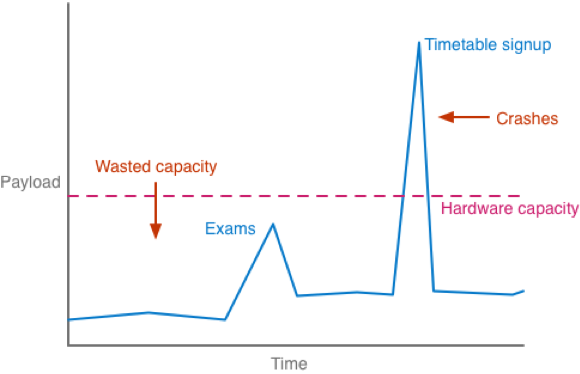
\includegraphics[width=3in]{CloudComputing_1.png}
\caption{Use of information system with fixed hardware capacity \label{fig:1}}
\end{figure}

Cloud computing would resolve this problem by scaling up for a couple of hours, and it would save money by scaling down during semester when the system is not used too heavily. Such cloud is called platform as a service.

Another cloud solution would be using an existing academic system, available as a service, where hosting is handled by the company that sells the system. 

\subsection{Infrastructure as a service}

Infrastructure services deliver computer hardware as a service. Clients, instead of having to purchase the infrastructure, pay regular fee to the provider to get scalable infrastracture.

An example of platform as a service is Amazon EC2:

\begin{quotation}
Amazon Elastic Compute Cloud (Amazon EC2) is a web service that provides resizable compute capacity in the cloud. It is designed to make web-scale computing easier for developers. \citep{amazon}
\end{quotation}

\subsection{Platform as a service}

Platform as a service is a whole platform moved to the cloud. 

\begin{quotation}
PaaS solutions are development platforms for which the development tool itself is hosted in the cloud and accessed through a browser. With PaaS, developers can build web applications without installing any tools on their computer and then deploy those applications without any specialized systems administration skills. \citep{paas}
\end{quotation}

An example of PaaS is Google App Engine.

\begin{quotation}
App Engine offers fast development and deployment; simple administration, with no need to worry about hardware, patches or backups; and effortless scalability. \citep{google_appengine}
\end{quotation}

\subsection{Software as a service}

Probably the most popular type of service cloud is software as a service. It’s a new model of selling software: Instead of selling individual versions, the provider hosts software and user data, giving user access from anywhere.

Hosting is usually outsourced to infrastructure provider, as described in the chapter. 